% -*- latex -*-

\documentclass{llncs}

% Prevents an error in the enumitem, which conflicts with a legacy thing in
% IEEEtran package.
%\let\labelindent\relax

\usepackage{amsfonts}
\usepackage{amssymb}
\usepackage[cmex10]{amsmath}
\usepackage{booktabs}
\usepackage{enumitem}
\usepackage{graphicx}
\usepackage{fancyvrb}
\usepackage{ifthen}
\usepackage{cite}
\usepackage[caption=false,font=footnotesize]{subfig}
\usepackage{tabulary}
\usepackage{url}
\usepackage{xspace}
\usepackage[pdfborder={0 0 0}]{hyperref}
\usepackage{verbatim}

\usepackage{color}
\definecolor{yellow}{rgb}{1,1,0}
\definecolor{black}{rgb}{0,0,0}
\definecolor{ltcyan}{rgb}{.75,1,1}
\definecolor{red}{rgb}{1,0,0}
\definecolor{gray}{rgb}{.6,.6,.6}
\definecolor{darkred}{rgb}{0.5,0,0}
\definecolor{darkgreen}{rgb}{0,0.5,0}

% Cite commands I use to abstract away the different ways to reference an
% entry in the bibliography (superscripts, numbers, dates, or author
% abbreviations).  \scite is a short cite that is used immediately after
% when the authors are mentioned.  \lcite is a full citation that is used
% anywhere.  Both should be used right next to the text being cited without
% any spacing.
\newcommand*{\lcite}[1]{~\cite{#1}}
\newcommand*{\scite}[1]{~\cite{#1}}

\newcommand{\etal}{et al.\xspace}

\newcommand*{\keyterm}[1]{\emph{#1}}

\newcommand{\fix}[1]{{\color{red}\textsc{[#1]}}}
%\newcommand{\fix}[1]{}

% Avoid putting figures on their own page.
\renewcommand{\textfraction}{0.05}
\renewcommand{\topfraction}{0.95}
\renewcommand{\bottomfraction}{0.95}

% Make sure this is big enough so that only big figures end up on their own
% page but small enough so that if a figure does have to be on its own
% page, it won't push everything to the bottom because it's not big enough
% to have its own page.
\renewcommand{\floatpagefraction}{.75}

% Allows multiline equations (align environment) to break across pages.
\allowdisplaybreaks[4]

\newenvironment{packed_itemize}{
  \begin{itemize}[noitemsep]
}{
  \end{itemize}
}


\begin{document}

\sloppy

%
% paper title
% can use linebreaks \\ within to get better formatting as desired
%\title{A Formal Metric for Large-Scale Parallel Algorithm Performance Analysis}
\title{Formal Metrics for Large-Scale Parallel Performance}


\author{Kenneth Moreland \and Ron Oldfield}
\institute{Sandia National Laboratories, Albuquerque, NM 87185, USA}


\maketitle


\begin{abstract}
Performance measurement of parallel algorithms is well studied and well
understood. However, a flaw in traditional performance metrics is that they
rely on comparisons to serial performance with the same input. This
comparison is convenient for theoretical complexity analysis but impossible
to perform in large-scale empirical studies with data sizes far too large
to run on a single serial computer. Consequently, scaling studies currently
rely on ad hoc methods that, although effective, have no grounded
mathematical models. In this position paper we advocate using a rate-based
model that has a concrete meaning relative to speedup and efficiency and
that can be used to unify strong and weak scaling studies.
\end{abstract}

\section{Introduction}

\noindent
Empirical scaling studies are an important component in the analysis of
parallel algorithms and systems. A scaling study tests the performance of a
parallel algorithm using different numbers of processing elements and
usually over different amounts of data. A good scaling study shows how
effectively additional processing elements are used by the algorithm and
through trends provides evidence of behavior at future larger scales.

The practice of measuring scaling relies on the well studied models for the
theory of parallel performance. However, current theoretic
models rely on comparisons with algorithm behavior on a single, serial
processing element. Empirically measuring serial behavior for sufficiently
large parallel problems is impractical.

\subsection{Performance Analysis Theory}

\noindent
The following is a brief overview of parallel algorithm performance.

The \keyterm{speedup} of a parallel algorithm is defined as
\begin{equation}
  S(n,p) = \frac{T^*(n)}{T(n,p)}
  \label{eq:Speedup}
\end{equation}
where $T(n,p)$ is the time it takes to run the parallel algorithm on $p$
processing elements with an input of size $n$, and $T^*(n)$ the time for the
best serial algorithm on the same input. The best possible serial algorithm
may be different than the parallel algorithm although using the same
algorithm is also common practice.

In theory the best possible speedup achievable is $S(n,p) =
p$\lcite{Faber1986} (although superlinear measurements can occur in
practice\lcite{Gustafson1990}). Thus, we measure the \keyterm{efficiency}
as the ratio of the observed speedup to the ideal speedup.
\begin{equation}
  E(n,p) = \frac{S(n,p)}{p} = \frac{T^*(n)}{p \; T(n,p)}
  \label{eq:Efficiency}
\end{equation}

Amdahl\scite{Amdahl1967} famously observes the limits of scaling any
parallel algorithm based on the fraction $f$ of inherently serial
computation that exists in any algorithm. The equation derived from this
observation is known as \keyterm{Amdahl's law}.
\begin{equation}
  S(n,p) \leq \frac{1}{f + (1-f)/p}
  \label{eq:Amdahl}
\end{equation}

Gustafson\scite{Gustafson1988} observes that the serial fraction tends to
go down for larger data sizes in parallel algorithms, which justifies the
use of parallel computing for large problems. The \keyterm{Gustafson-Barsis
  law} reformulates speedup in terms of the parallel execution rather than
the serial execution.
\begin{equation}
  S(n,p) \leq p + (1-p) \cdot s(n,p)
  \label{eq:GustafsonBarsis}
\end{equation}
where $s(n,p)$ is the fraction of time in the parallel execution performing
sequential operations. This law shows that speedup can be increased
indefinitely as long as the serial fraction drops commensurately with the
processing element increase, which can often be done by increasing the
problem size. Grama \etal\scite{Grama1993} introduce an
\keyterm{isoefficiency} relation that determines how much a problem needs to
grow to maintain a desired level of efficiency. Given a desired efficiency
$E_d$, the following inequality must hold.
\begin{equation}
  T(n,1) \geq \frac{E_d}{1-E_d} T_o(n,p)
  \label{eq:Isoefficiency}
\end{equation}
where $T_o(n,p)$ is the total overhead (redundant, idle, and extra
computation plus communication) for running the algorithm on $p$ processing
elements for data of size $n$.

Performance analysis theory is reviewed in much more detail in many
parallel computing textbooks such as Quinn's\scite{Quinn2004}.

\subsection{Limitations of Performance Analysis}

\noindent
Although our definition for speedup and its derived quantities work well
for theoretical complexity analysis, they all rely in some way on knowing
the serial performance. With large-scale simulations today reaching orders
of billions to trillions of
elements\lcite{Bernaschi2013,Rossinelli2013,Bussmann2013,Habib2013},
directly measuring serial performance is often impossible. The Gustafson-Barsis
law needs only the serial fraction, but estimates for serial
fraction such as the \keyterm{Karp-Flatt} metric\lcite{Karp1990} require
knowing the serial performance anyway.

%% Because of this issue, many studies attempt to assess scalability directly
%% from an algorithm's running time relative to the number of processing
%% elements, which is called \keyterm{strong scaling}\lcite{Kaminsky2015}.
%% Because a parallel algorithm with perfect speedup has a running time
%% proportional to $1/p$, we look for time behavior that follows a roughly
%% hyperbolic plot that asymptotically approaches a number close to zero
%% (representing the overhead). However, all but the very worst scaling
%% algorithms tend to asymptotically approach some constant time, which makes
%% it difficult to distinguish when an algorithm is actually scaling
%% well. Often we try to rectify the problem by plotting the running time
%% using log scaling for both the number of processing elements and the time
%% because perfect scaling on this plot is a straight line.

%% However, overheads of any polynomial order are also straight lines. A
%% scaling study compares against the ideal performance, which has polynomial
%% order of 1 (or -1 when plotting by time). A trend with an order as low as 2
%% still has serious scaling limitations. Visually differentiating slopes this
%% close can be challenging and can depend on the dimensions of the
%% plot\lcite{Cleveland1994}. Consequently, the log axes make it difficult to
%% differentiate good and bad scaling.

%% Another common approach is to measure \keyterm{weak scaling}\lcite{Kaminsky2015}.
%% In weak scaling the size of the input data is increased with the number of
%% processing elements. Typically the input is kept proportional to the number
%% of processing elements. In this case a perfectly scaling algorithm will
%% have the same running time for all experiments. Although an important
%% characteristic, weak scaling should also be coupled with strong scaling to
%% get a complete picture. Also, analyzing weak scaling this way requires the
%% ability to vary the data proportionally with the processing elements, which
%% is not always possible.  For example, some simulations might adaptively
%% remesh based on some criteria, which means the size of the data can be
%% modified but not directly set by an analyst.

Because of this issue, most studies attempt to asses scalability with a
pair of trends named strong scalability and weak
scalability\lcite{Kaminsky2015}. \keyterm{Strong scaling} demonstrates an
algorithm's behavior by measuring its run time on a particular data set for
various numbers of processing elements. Perfect strong scaling has a
running time proportional to $1/p$. As we shall see in examples later, it
is difficult to compare the quality of plotted curves to this perfect
hyperbolic on both linear and log scales.

Per Amdahl's law, there are inevitable limits to strong scaling. In
contrast \keyterm{weak scaling} varies the problem size proportionally with
the number of processing elements. It may not always be possible to keep
the problem size proportional to the job size, which make weak scaling more
difficult. The metrics advocated in this paper simplify studying
scalability by removing the dependence between problem size and number of
processing elements. We encourage using them to sample the 2D parameter
space of problem size and number of processing elements as widely as
possible for a broader view of the scalability.

Some studies use an ad hoc version of speedup or efficiency that replaces the
immeasurable $T^*(n)$ with some arbitrarily chosen measurement, usually the
time run on the smallest number of processing elements. The problem with
this approach is that the absolute meaning of ``speedup'' and
``efficiency'' changes between experiments in a study. Furthermore, the
metric cannot be used in weak scaling because the problem size is not held
constant.

Finally, some studies use rate in terms of the size of input computed per
unit time rather than absolute run time to assess
scalability\lcite{Kaminsky2015}. Rate is formally defined as
\begin{equation}
  R(n,p) = \frac{n}{T(n,p)}
  \label{eq:Rate}
\end{equation}
Some analysts have discovered that rate, being essentially a reciprocal of
time, provides a much better visual analysis of scaling, and it is
an essential mechanism advocated in this position paper.

This paper establishes a more pragmatic definition and efficiency that can
be easily measured empirically. Furthermore, we demonstrate how rate can be
used as a proxy for speedup and can unify strong and weak scaling to
provide a more complete analysis. These metrics are demonstrated using real
performance data.


\section{Deriving Efficiency from Cost Analysis}
\label{sec:CostAnalysis}

\noindent
In this section we will use \keyterm{cost}, a metric that is simple to
measure, to define efficiency in lieu of the immeasurable speedup. Cost is
intuitively the number of processing elements used multiplied by the amount
of time they are used.
\begin{equation}
  C(n,p) = p \; T(n,p)
  \label{eq:Cost}
\end{equation}
Cost is sometimes used in theoretical algorithm analysis\lcite{JaJa1992}
and is often used for HPC allocations, which are typically measured in
core-hours.

Clearly the most efficient algorithm will be the one that costs the least
to run. Although we expect the cost to go up with the problem size, a
perfectly scaled algorithm on a fixed input size will cost the same
regardless of how many processors are used. That is, adding processors
reduces the time proportionally. Given a strong scaling study on a problem
of a particular size, we can identify the best (minimal) cost, $C^*(n)$,
that uses $p^*$ processing elements. With this best cost we can redefine
efficiency as the ratio of this best cost to the actual cost.
\begin{equation}
  E(n,p) = \frac{C^*(n)}{C(n,p)}
  \label{eq:EfficiencyCost}
\end{equation}

If we make the typical assumptions that the minimal cost is when the serial
algorithm is run ($C^*(n) = T^*(n)$), then we observe that
Equation~\ref{eq:EfficiencyCost} simplifies to
Equation~\ref{eq:Efficiency}, making this definition of efficiency
equivalent but broader than the traditional definition. And unlike the
traditional definition of efficiency, determining efficiency from cost is
straightforward at large scales.


\section{Strong and Weak Scaling with Cost Per Unit}
\label{sec:CostPerUnit}

\noindent
Our previous definition of efficiency (Equation~\ref{eq:EfficiencyCost})
works well for strong scaling where the data size is constant, but cannot
be compared across different data sizes for weak scaling. To describe
efficiency under weak scaling we define the new metric \keyterm{cost per
  unit}, $C_{/u}$. Cost per unit is the amortized computational cost for
one unit of data.
\begin{equation}
  C_{/u}(n,p) = \frac{C(n,p)}{n} = \frac{p \; T(n,p)}{n}
  = \frac{p}{R(n,p)}
  \label{eq:CostPerUnit}
\end{equation}

The important feature of cost per unit is that under perfect scaling the
cost per unit is constant under any number of processing elements \emph{or}
data sizes. Thus, given multiple strong scaling studies over data of
different sizes, we can find the best (minimal) cost per unit $C_{/u}^*$,
that uses $p^*$ processing elements operating on data of size $n^*$.
With this best
cost per unit we can adjust the efficiency to be comparable across all
possible configurations.
\begin{equation}
  E(n,p) = \frac{C_{/u}^*}{C_{/u}(n,p)}
  \label{eq:EfficiencyCostPerUnit}
\end{equation}

With this definition of efficiency we can combine strong and weak scaling
studies into one unified analysis.

\section{Rate as a Proxy for Speedup}
\label{sec:RateProxy}

\noindent
Both efficiency and speedup are good metrics for parallel performance
analysis. However, many analysts prefer using speedup, particularly for
visual (chart) analysis. This is because good scaling shows an upward
sloping speedup as jobs get larger whereas even a good scaling algorithm
will show a gradual drop-off from a perfect efficiency of 1.

Although there is no way to compute the speedup at large scales, we can
show that rate (Equation~\ref{eq:Rate}) is a valid proxy for speedup. If we
substitute rate for time in Equation~\ref{eq:Speedup}, we get the
following.
\begin{equation}
  S(n,p) = \frac{T^*(n)}{T(n,p)} = \frac{T^*(n)}{n} R(n,p)
  \label{eq:SpeedupFromRate}
\end{equation}

We can observe that for a given problem size (i.e. $n$ held constant) the
speedup is proportional to the rate. This means that the rate curve will
have the exact same shape as the speedup curve, and visually they will be
identical with the appropriate scaling of the ordinate axis.

For a proper parallel performance analysis we need to compare our measured
metrics with the ideal metrics. These ideal values are implicit in the
definition of efficiency ($E_\mathrm{ideal}(n,p) = 1$) and speedup
($S_\mathrm{ideal}(n,p) = p$).
%% The ideal rate is dependent on the measured
%% best cost per unit and can be derived from
%% Equation~\ref{eq:EfficiencyCostPerUnit}.
%% \begingroup
%% \addtolength{\jot}{1ex} % Space equations a bit more. Fractions are cluttered.
%% \begin{align}
%%   \frac{C_{/u}^*}{C_{/u}(n,p)} &= E(n,p) \nonumber \\
%%   C_{/u}^* \frac{n}{p \; T(n,p)} &= E(n,p) \nonumber \\
%%   \frac{C_{/u}^*}{p} R(n,p) &= E(n,p) \nonumber \\
%%   \frac{C_{/u}^*}{p} R_\mathrm{ideal}(n,p) &= 1 \nonumber \\
%%   R_\mathrm{ideal}(n,p) &= \frac{p}{C_{/u}^*}
%%   \label{eq:IdealRate}
%% \end{align}
%% \endgroup
The ideal rate can be derived from Equation~\ref{eq:EfficiencyCostPerUnit}
by substituting the cost per unit with the rate
(Equation~\ref{eq:CostPerUnit}) and solving for rate when the efficiency is
the optimal value of 1.
\begin{equation}
  R_\mathrm{ideal}(n,p) = \frac{p}{C_{/u}^*}
  \label{eq:IdealRate}
\end{equation}

Note that the curve for $R_\mathrm{ideal}(n,p)$ is independent of $n$,
which means we can use the same ideal rate for both strong and weak scaling
analysis and can compare these rates with each other.

%% \section{Effective Empirical Parameter Sampling}

%% Both the efficiency (Equation \ref{eq:EfficiencyCostPerUnit}) and the ideal
%% rate (Equation \ref{eq:IdealRate}) are defined in terms of the optimal cost
%% per unit, $C_{/u}^*$. Finding the optimal cost per unit is imperative to
%% understanding scaling with these metrics. With any empirical study the best
%% known cost per unit is constrained to the values measured by experiment.
%% The quality of the measured optimal cost per unit can be undermined by a
%% narrow exploration of parameters, but then so is a scaling study as a
%% whole. A quality scaling study measures a wide breadth of parameters.

%% Most scaling studies must consider at least two parameters: the size of the
%% problem and the number of processing elements. Traditional strong and
%% weak scaling studies limit the search to a 1D line in this 2D parameter
%% space; strong scaling explores the line where the problem size is set to a
%% constant value, and weak scaling explores the line where the problem size
%% and number of processing elements are proportional. Such one dimensional
%% analysis is a sparse sampling of the parameter space that can easily miss
%% optimal configurations.

%% Instead, the cost-per-unit--based efficiency and rate metrics encourage
%% sampling the two dimensional parameter space of problem size and processing
%% elements. A more thorough parameter sampling of this nature lends more
%% credibility in the results of the scaling study.


\section{Examples}

\noindent
In the previous sections we provide mathematical derivations to show how
to use rate as a proxy for speedup and to use cost per unit to find the
efficiency and ideal rate across all scales. In this section we demonstrate
using these metrics on real measured data. We can observe that the metrics
of rate and efficiency make it easier to visually identify the behavior and
trends at different scales of processing elements.

\subsection{Gordon Bell Finalist}

\noindent
Our first data set comes from a study by Habib \etal\scite{Habib2013}, which is
one of the 2013 Gordon Bell finalists. We choose this source because in
addition to showing impressive scaling, the authors make many measurements
across many scales and report the results completely enough to extract the
information and continue analysis. In particular, we look at the
performance data for scaling the full HACC code on Titan (Section~4.3.2 in
the original paper).

Figure~\ref{fig:HabibTraditional} shows the performance data from the
strong and weak scaling studies using a traditional time plot. The curves
for the data are very similar for what we would expect for perfect scaling:
a hyperbolic curve for strong scaling and a horizontal line for weak
scaling. Habib \etal also provide an ad hoc metric of time over data size
to unify the curve shape of the two plots, which is also replicated in
Figure~\ref{fig:HabibTraditional}. Again, both curves appear close to
perfect.

\begin{figure}[htb]
  \centering
  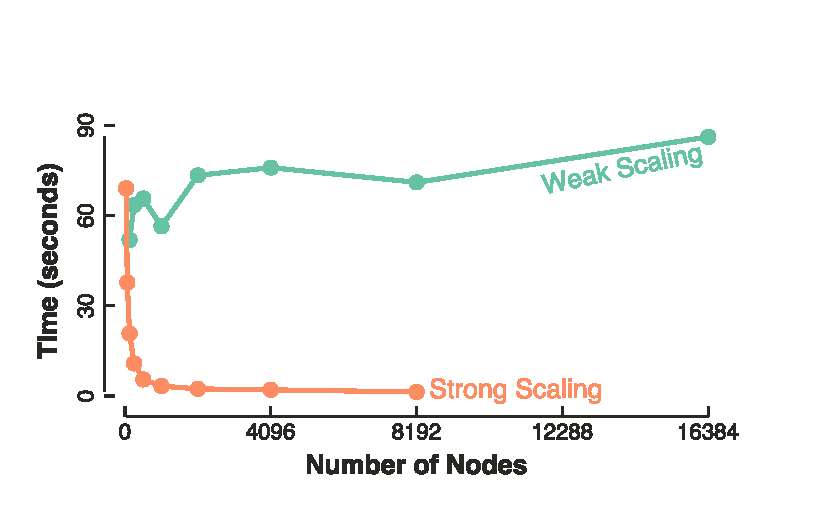
\includegraphics[width=.48\linewidth]{images/HabibTime}\quad
  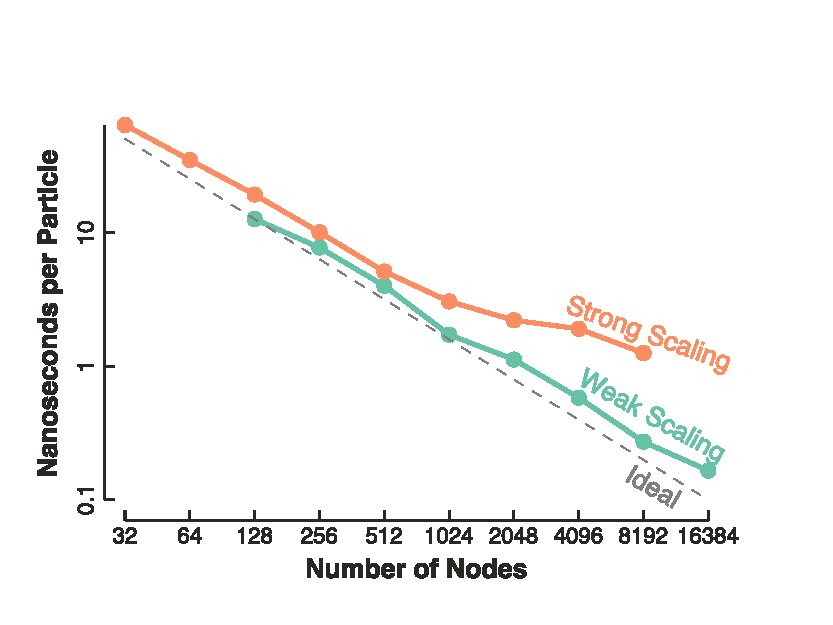
\includegraphics[width=.48\linewidth]{images/HabibTimePerParticle}
  \caption{Data from the Habib \etal\scite{Habib2013} Gordon Bell
    finalist. The left chart shows the data using a traditional time
    metric. The right chart replicates the presentation of Figure~3 in the
    original paper using an ad hoc metric and a log-log
    scale. Both charts present the data in a way to suggest near perfect
    scaling for both scaling studies.}
  \label{fig:HabibTraditional}
\end{figure}

Figure~\ref{fig:HabibBetter} shows the same data using the rate and
efficiency metrics advocated in this paper. The weak scaling is shown to
diverge from ideal by a measurable fraction, which is to be expected when
scaling over 3 orders of magnitude. The strong scaling study is shown to
diverge very far from ideal.

\begin{figure}[htb]
  \centering
  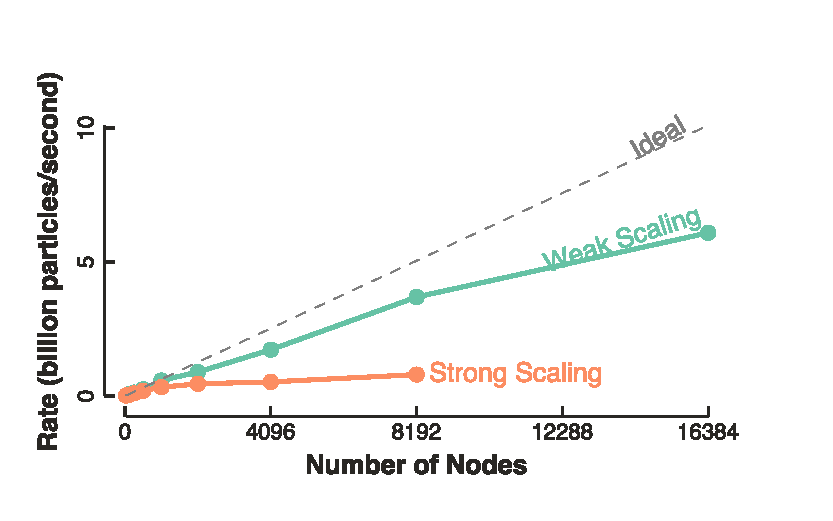
\includegraphics[width=.48\linewidth]{images/HabibRate}\quad
  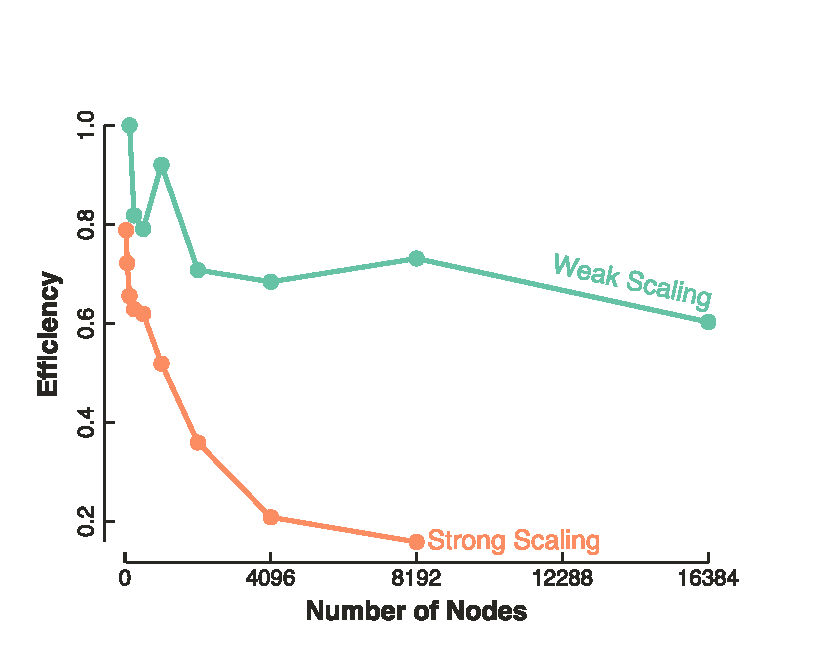
\includegraphics[width=.48\linewidth]{images/HabibEfficiency}
  \caption{Data from the Habib \etal\scite{Habib2013} Gordon Bell finalist
    using the rate (left) and efficiency (right) metrics advocated in this
    paper. These plots give a more realistic and visually measurable
    representation of scaling than the charts in
    Figure~\ref{fig:HabibTraditional}.}
  \label{fig:HabibBetter}
\end{figure}

%% Please note that it is not our intention to criticize the scaling shown by
%% Habib \etal\scite{Habib2013}. On the contrary, they show HACC to be world
%% class in scalability and demonstrate a consistent efficiency while scaling
%% the problem by an order of magnitude. Rather, our intention is to present
%% these data in a more informative way.

\subsection{Imperfect Scaling}

\noindent
Our second data set comes from a study by Oldfield
\etal\scite{Oldfield2014}. In this study a visualization
algorithm has a high communication overhead and therefore has a known limit
on its scalability. The study shows how transferring data between parallel
jobs of different sizes can sometimes be faster than combining both in one
large job.

A traditional plot of the time of the visualization component shown in
Figure~\ref{fig:OldfieldTraditional} gives curves that suggest good scaling
performance. However, when we show the same data using the rate and
efficiency metrics, shown in Figure~\ref{fig:OldfieldBetter}, we can
clearly see the effect the communication overhead has on the scalability of
the algorithm. Without such a presentation, erroneous interpretation of the
performance is sure to occur.

\begin{figure}[htb]
  \centering
  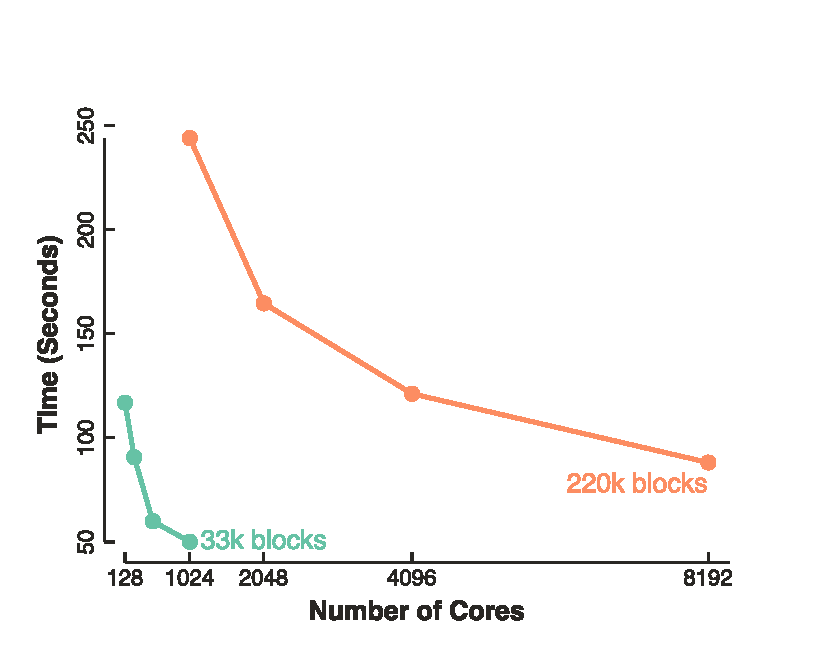
\includegraphics[width=.48\linewidth]{images/OldfieldTimeLinear}
  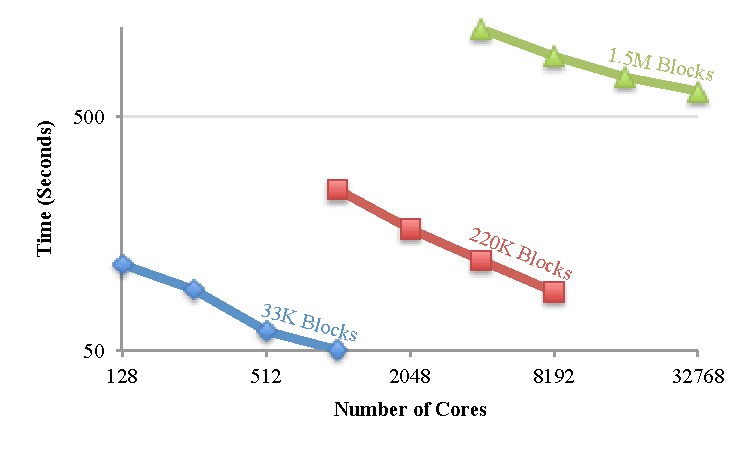
\includegraphics[width=.48\linewidth]{images/OldfieldTimeLog}
  \caption{Data from the Oldfield \etal\scite{Oldfield2014}
    simulation-visualization integration study where the visualization
    (shown here) has a high communication overhead. These plots use the
    traditional method of showing the trend of run time using linear and
    log-log scaling.}
  \label{fig:OldfieldTraditional}
\end{figure}

\begin{figure}
  \centering
  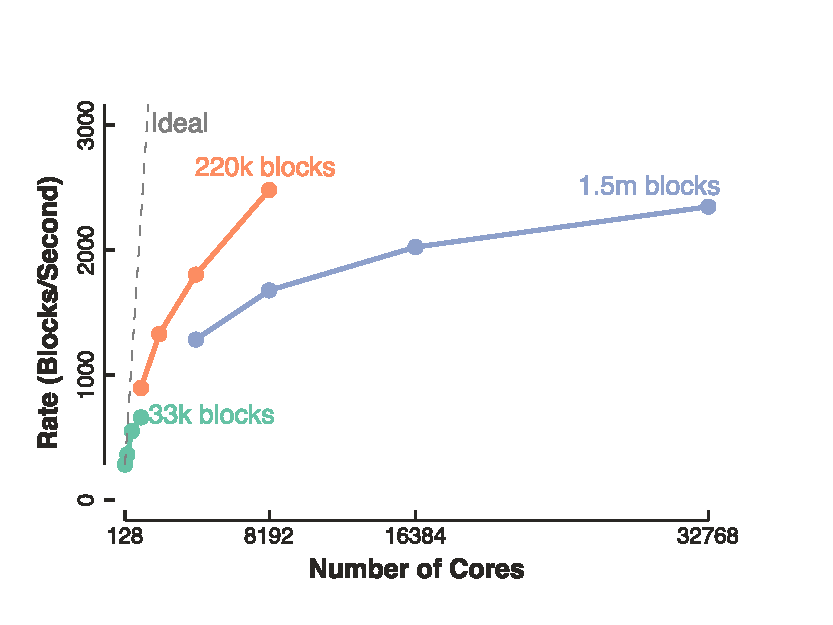
\includegraphics[width=.48\linewidth]{images/OldfieldRate}\quad
  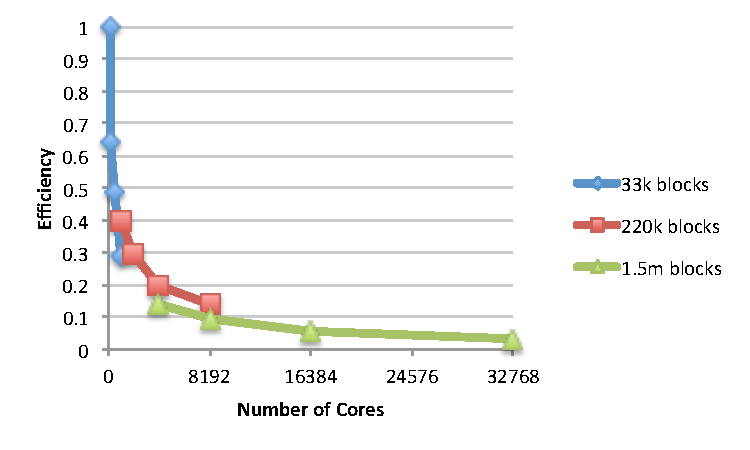
\includegraphics[width=.48\linewidth]{images/OldfieldEfficiency}
  \caption{Data from Oldfield \etal\scite{Oldfield2014} using
    rate (left) and efficiency (right) to reveal that the communication
    overhead has a severe impact on the overall scalability.}
  \label{fig:OldfieldBetter}
\end{figure}

\section{Discussion}

\noindent
In this paper we discuss limitations of traditional parallel performance
analysis and problems with the current metrics often used. We provide
derivations of rate as a proxy for speedup, ideal rate, and efficiency and
demonstrate with real data how these provide accurate visual
representations of scalability. As scientists, we should demand this high
level of transparency and honesty in performance analysis.

With these observations, we provide the following recommendations for the
visual display of parallel performance.
\begin{packed_itemize}
\item Do not rely on running time for performance analysis. Instead use
  rate, efficiency, or both.
\item Avoid using log-log scaling on plot axes, which hides major
  inefficiencies. If necessary repeat linear plots at different scales.
\item Rather than performing separate weak and strong scaling studies,
  incorporate them in one. Perform several strong scaling studies at
  different scales. Then find an overall minimal cost per unit and plot all
  the measurements together as demonstrated in the figures in this paper.
\end{packed_itemize}

%% As architectures continue to advance, many are beginning to advocate
%% measuring power instead of or in addition to speed\lcite{Cameron2012}. As
%% future work we advocate using a cost model for this as well, which should
%% provide a similarly effective cost per unit for efficiency (although rate
%% may lose meaning).

The use of rate or efficiency to measure parallel performance is not itself
a new technique. After all, the ubiquitous ``FLOPS'' measurement is itself
a rate, and measurements given in data unit per time unit can be found
throughout the literature. However, other metrics of varying effectiveness
are also found in published material with little or no justification for
the choice. The decision for scaling metrics should not be arbitrary; it
can have enormous impact on the viability of the analysis. Our intention is
to show that the metric visualized does matter, to provide a best practices
for measuring scalability, and to explain why these metrics work better
than others.


% use section* for acknowledgement
\section*{Acknowledgment}

\noindent
This material is based in part upon work supported by the U.S. Department
of Energy, Office of Science, Office of Advanced Scientific Computing
Research, Scientific Discovery through Advanced Computing (SciDAC) program
under Award Number 12-015215.

Sandia National Laboratories is a multi-program laboratory managed and
operated by Sandia Corporation, a wholly owned subsidiary of Lockheed
Martin Corporation, for the U.S. Department of Energy's National Nuclear
Security Administration under contract DE-AC04-94AL85000. \hfill
{\footnotesize SAND 2014-16181C}

\bibliographystyle{splncs03}
\bibliography{FormalScalingMetric}

\end{document}


